\section{SMDA Interface}
\label{sect:smda_interface}

The iPad version of the SMDA tool allows the user to both enter input data and
view the results. Input is done through a table-based user interface. The
results are shown as a series of graph views. (For more information about SMDA,
see section \ref{sect:background_smda}.)

The ``Experimental SMDA Tool'' button on the home screen takes the user to a
list of measurements. \mawapp with two example result sets to help the user get
accustomed to the interface.

\subsection{Input}
\label{sect:smda_interface_input}

Tapping one of these measurement lists switches to the screen shown in figure
\ref{fig:screenshot_smda_list}. There is one section on this screen for each
type of input to the SMDA algorithm: pathway, transport process, reaction,
pathway as reaction, and measurement.

\begin{figure}[htb]
    \center{
        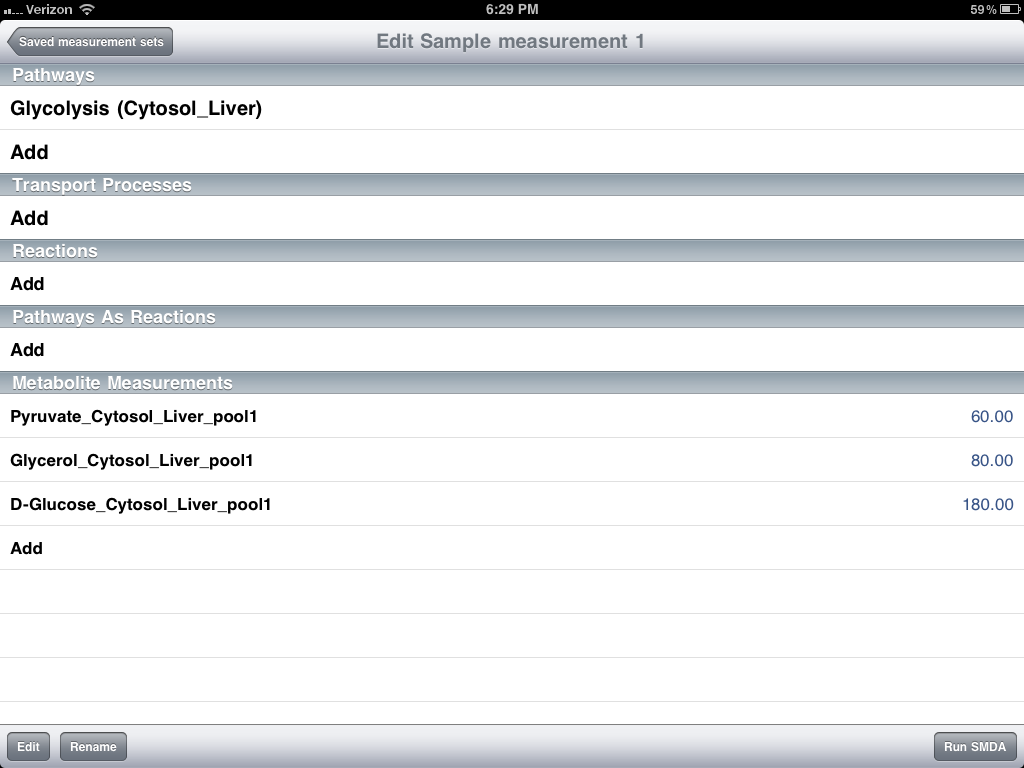
\includegraphics[width=\textwidth]{maw/figures/screenshot_smda_list}}
    \caption{\label{fig:screenshot_smda_list} List of measurements in SMDA}
\end{figure}

\begin{figure}[htb]
    \center{
        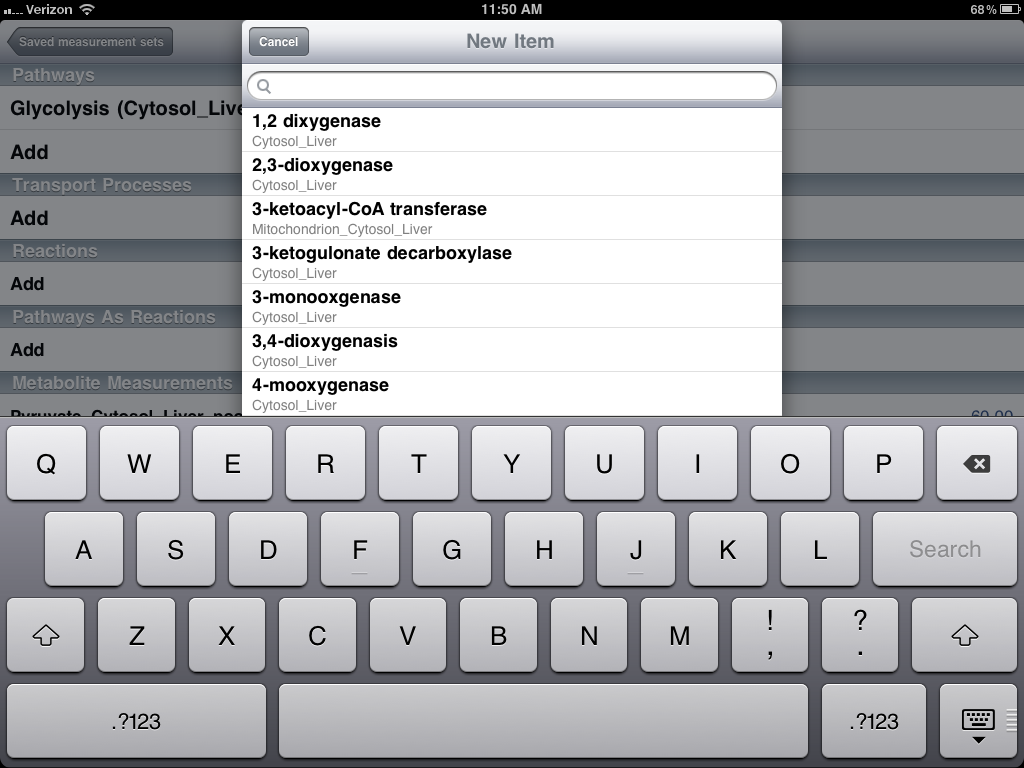
\includegraphics[width=\textwidth]{maw/figures/screenshot_smda_add_reaction}}
    \caption{\label{fig:smda_add_reaction} Adding a reaction in SMDA}
\end{figure}

\begin{figure}[htb]
    \center{
        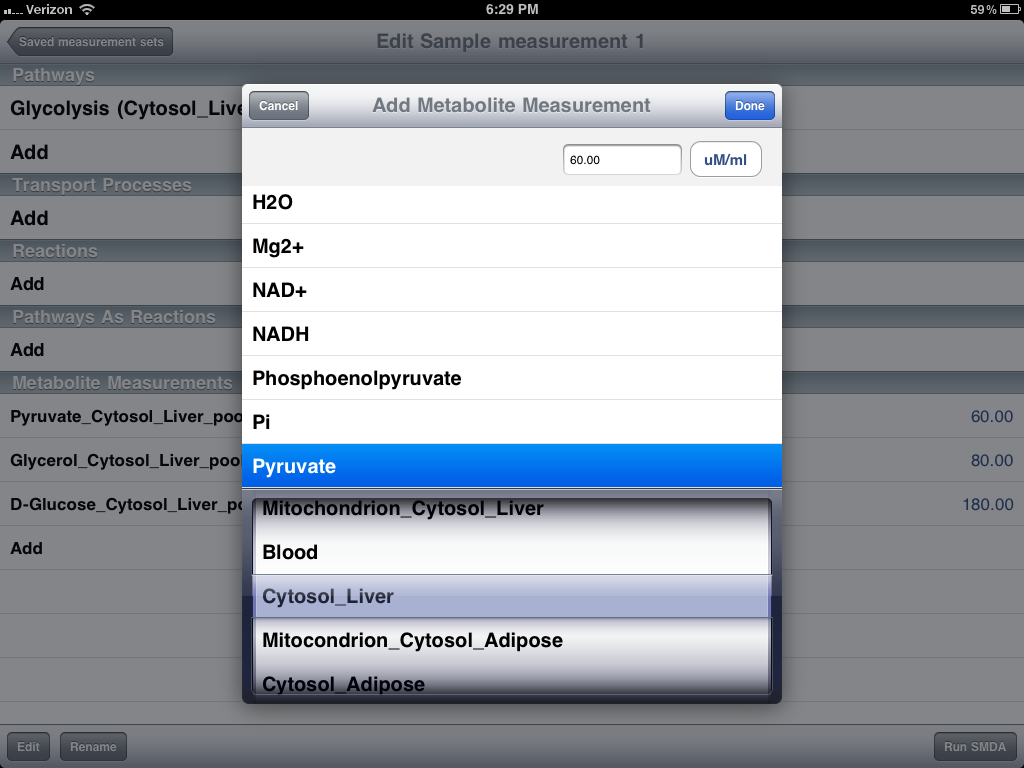
\includegraphics[width=\textwidth]{maw/figures/screenshot_smda_edit_measurement}}
    \caption{\label{fig:smda_edit_measurement} Editing a measurement in SMDA}
\end{figure}

New input parameters can be added by tapping the ``Add'' row in any of the
sections. Figure \ref{fig:smda_add_reaction} shows the screen for adding a new
reaction. Tapping an existing row brings up the same screen, allowing the user
to change their selection.

Figure \ref{fig:smda_edit_measurement} shows a similar screen for editing
measurements.

To better explain this interface, here is a simple example. The application
includes two sample measurements. \textbf{Sample Measurement 1} measures
metabolites in the pathway \textbf{Glycolysis} in the \textbf{Cytosol\_Liver}
compartment. These metabolites are \textbf{Pyruvate} ($60 \mu M/ml$),
\textbf{Glycerol} ($80 \mu M/ml$), and \textbf{D-Glucose} ($180 \mu M/ml$).

To select a pathway, the user taps the ``Add'' row of the ``Pathways'' section
of the table. A view appears with a list of pathways. The user taps ``Glycolysis
(Cytosol\_Liver)'' to select it and it appears in the ``Pathways'' section.

To add measurements, the user taps the ``Add'' row of the ``Metabolite
Measuremnents'' section and the view in figure \ref{fig:smda_edit_measurement}
appears so the user can select Pyruvate and enter $60 \mu M/ml$. This process is
repeated for Glycerol and D-Glucose.

It is necessary to input the pathways before any metabolite measurements because
the metabolite list contains only metabolites that are members of the given
pathways.

\subsection{Output}
\label{sect:smda_interface_output}

The interface for browsing SMDA results is very similar to the one for looking
at a normal pathway. There are two main differences. The first, shown in figure
\ref{fig:smda_results}, is the bottom toolbar that provides buttons to move
forward and backward in the list of scenarios.

\begin{figure}[htb]
    \center{
        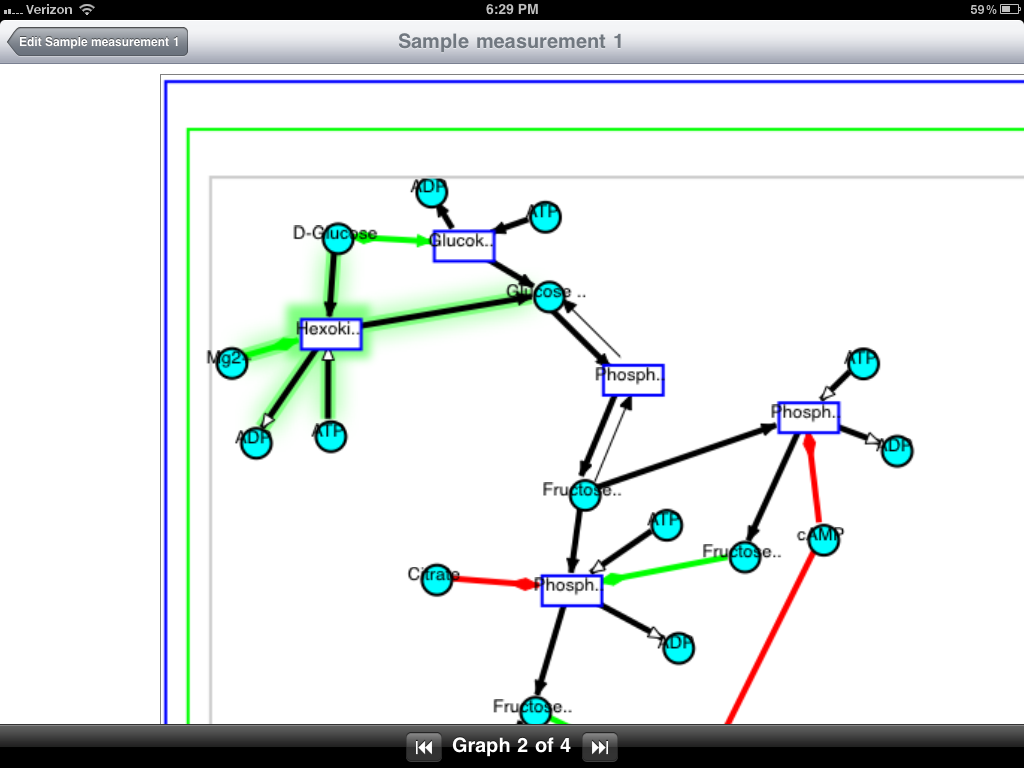
\includegraphics[width=\textwidth]{maw/figures/screenshot_smda_results}}
    \caption{\label{fig:smda_results} One scenario in an SMDA result set}
\end{figure}

The second difference, shown in figure \ref{fig:smda_results_highlight}, is the
green highight shown behind edges coming out of a reaction if that reaction is
in a different active/inactive state from the previously viewed scenario. In
this example, ``Triose...'' was inactive in scenario 1 but active in scenario 2.
Flipping between the two scenarios will keep this reaction highlighted.

\begin{figure}[htb]
    \center{
        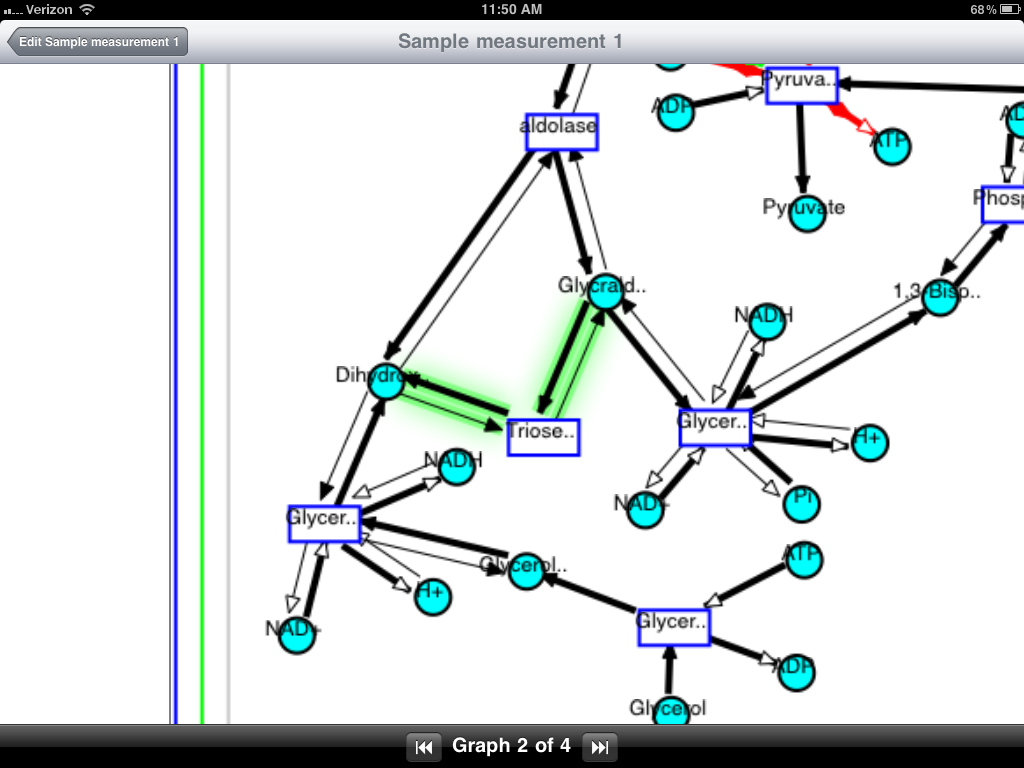
\includegraphics[width=\textwidth]{maw/figures/screenshot_smda_results_highlight}}
    \caption{\label{fig:smda_results_highlight} Zoomed view of a highlighted
    reaction in an SMDA scenario}
\end{figure}
